%%%%%%%%%%%%%%%%%%%%%%%%%%%%%%%%%%%%%%%%%%%%
\chapter{Data Acquisition}
%%%%%%%%%%%%%%%%%%%%%%%%%%%%%%%%%%%%%%%%%%%%
\begin{center}
  \begin{minipage}{0.75\textwidth}
    \begin{small}
      “I went to the woods because I wished to live deliberately, to front only the essential facts of life, and see if I could not learn what it had to teach, and not, when I came to die, discover that I had not lived”.\\
      \null\hfill\emph{Walden. Henry David Thoreau}
    \end{small}
  \end{minipage}
  \vspace{0.5cm}
\end{center}

Images were acquired using a digital microscope through various polarization filter arrangements to determine each materials polarization and texture properties.  A broadband white light source was utilized to illuminate the target under investigation.  The DOP of the light source was found to be low /(<.02%/) The lights within the room were turned off during data acquisition to reduce the amount of ambient light noise [TODO explain how this would be handled outside a lab setting].  A custom web application was created to capture, label and store images for easy access and processing.  The acquired data and processing code can be found in [17].

%%%%%%%%%%%%%%%%%%%%%%%%%%%%%%%%%%%%%%%%%%%
\section{Measurement of Stokes Parameters}
%%%%%%%%%%%%%%%%%%%%%%%%%%%%%%%%%%%%%%%%%%%
The Stokes parameters for a beam of light can be determined by measuring the flux values of orthogonal polarization states.  A variety of optical setups can be required to measure all of the Stokes parameters.  A Classical polarimeter is one that utilizes a rotating quarter wave plate in front of a linear polarizer to sample a sine wave from the intensities recorded by a detector.  A Fourier analysis is then performed on this signal to determine all of the Stokes parameters.

It is shown in [7] that the Stokes parameter of a beam can be generally calculated as
%
\begin{align}
    \mathbf{S} =
    \begin{bmatrix}
        S_0 \\
        S_1 \\
        S_2 \\
        S_3
    \end{bmatrix}
    =
    S_0
    \begin{bmatrix}
        P_H + P_V \\
        P_H - P_V \\
        P_P - P_M \\
        P_R - P_L
    \end{bmatrix}
\end{align}
%
where $P_H, P_V, P_P, P_M, P_R$ and $P_L$ represent flux measurements recorded through filters that extinguish orthogonal polarization states.

For most natural and man made objects the reflections are assumed to contain little or no circular polarization. The last row of the Stokes vector is therefore left out of the discussion and the equation becomes
%
\begin{align}
    \mathbf{S} =
    \begin{bmatrix}
        S_0 \\
        S_1 \\
        S_2
    \end{bmatrix}
    =
    S_0
    \begin{bmatrix}
        P_H + P_V \\
        P_H - P_V \\
        P_P - P_M
    \end{bmatrix}
\end{align}
%
The linear elements of the Stokes vector can be determined using just a linear polarizer and rotating the polarizer to 0, 45 90 and 135 degrees as seen in Figure xx.  These measurements are denoted $P_H, P_P, P_V,$ and $P_M$. They are the captured time average intensities for the $S$ and $P$ components of the electric field previously described.
%
%ßß\begin{center}
%  \makebox[\textwidth]{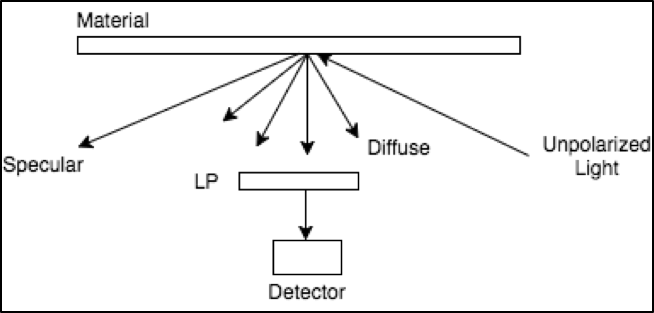
\includegraphics[width=8cm]{Sources/Background/Data_Acquisition/exper_setup.png}}
%\end{center}
%
The linear polarizer was calibrated using a polarizer of known axis orientation.  The calibration polarizer was kept with its axis constant to the S plane of the material.  The lens of the measurement polarizer was rotated until a null intensity was reached and the axis of transmission for the polarizer was orthogonal to that of the calibration polarizer.  The polarizer has a known extinction ratio of 19 and a polarization of 95% efficiency.  The spectral response across the visible spectrum is shown in Figure 12.  It shows that the polarizer produces a constant response across the visible range of the energy spectrum.

% TODO insert image of polarizer characteristics
When unpolarized light is incident, the Stokes vector for the exiting beam is identical to the polarizance of the Mueller matrix for the material and can be useful for classification of materials.

The intensity measurement is recorded with a detector.
%[TODO show work on S_out=MS_in]

%%%%%%%%%%%%%%%%%%%%%%%%%%%%%%%%%%%%%%%%%%%
\section{Single and Multi-Pixel Detectors}
%%%%%%%%%%%%%%%%%%%%%%%%%%%%%%%%%%%%%%%%%%%
For centuries the only photo detector available to those in the field of optics was the human eye.  Many methods were only capable of producing measurements via a null intensity method, where light was extinguished to determine orthogonality between polarization and polarizer transmission axes.  Modern single pixel photo detectors allow for the capturing of intensity or tone.  There are numerous types of detectors available made with different materials that exhibit different properties when interacting with light.  Silicon is a common substrate.

A single pixel is not enough to capture texture.  Multiple measurements need to be made using a single pixel in order to quantify a region of space around the surface, denoted by the units of steradians in the BRDF models.  Multi-pixel detectors with a larger field of view allow for multiple features and texture to be captured in an image.

A camera is made up of a pattern of multiple silicon photo detectors and filters.  The most common filter arrangement is that of a Bayer filter.  This pattern consists of red, green, and blue spectral filters arranged as shown in Figure 13.
%TODO insert image of Bayer filter

The individual intensities from each of these filters are combined with the camera to create a 3 channel RGB representation of the image scene.  Each channel represents the intensity of a given pixel for the color filter in the Bayer pattern.

Single and multi-pixel devices have been utilized in Polarimetry for different applications.  A camera was utilized for these experiments as it provides information on texture, as well as an ability to distinguish features in each of the spectral color channels.

The intensity values for each RGB channel of an image can easily be extracted using the OpenCV python package.  Note that OpenCV actually holds images in reverse order as BGR.  A typical graph of the quantum efficiency for each wavelength in the visible region for CMOS sensors typically used in consumer cameras, can be found in Figure 14.
% TODO insert bayer filter transmission characteristics

OpenCV, a popular image processing library in Python, stores images as intensities in a multidimensional array representing the blue, green, and red response curves shown above.  It is possible to separate these channels and perform a pseudo-spectral analysis.

%%%%%%%%%%%%%%%%%%%%%%%%%%%%%%%%%%%%%%%%%%%
\section{Determining Relative Water Content}
%%%%%%%%%%%%%%%%%%%%%%%%%%%%%%%%%%%%%%%%%%%
The steps for determining the RWC involve weighing the leaf in its current water state, artificially hydrating the leaf to its maximum capacity and completely drying out the leaf.  The procedure for obtaining the measurements necessary for obtaining the RWC are as follows [9,10],

1.	Remove leaf from host plant leaving approximately 2 cm of petiole

2.	Weigh leaf to acquire the Fresh Leaf Weight (FW)

3.	Place leaf petiole in solution of distilled water and CaCl2 at 2mM for at least 8 hours

4.	Weigh leaf to acquire Turgid Weight (TW)

5.	Place leaf in an oven at 60oC for 4 days

6.	Weigh leaf to acquire the Dry Weight (DW)


The relative water content can then be calculated as a percentage,
%
\begin{align}
    RWC = \frac{FW - DW}{TW - DW} x 100%
\end{align}
%
Note that the scale used for weighing needs to have at least 4 decimal places to ensure the accuracy of the measurements. Drying times and artificial hydration times can vary with species and oven temperature. An example of measurements can be found in Table 4.1.  All acquired RWC data can be found in the Appendix.
%
\begin{table}[htb]
  \centering
  \begin{tabular}{lllll}
    \toprule
    \textbf{Leaf} & \textbf{TFW} & \textbf{TW} & \textbf{DW} & \textbf{RWC} \\
    \midrule
      \texttt{11} & 2.7931 & 2.8335 & 0.2472 & 98.4379 \\
      \texttt{12} & 2.0883 & 2.1184 & 0.1876 & 98.4411 \\
      \texttt{21} & 1.7804 & 1.8051 & 0.1376 & 98.5187 \\
      \texttt{22} & 1.7655 & 1.8022 & 0.1404 & 97.7916 \\
      \texttt{31} & 2.1874 & 2.2359 & 0.1656 & 97.6573 \\
      \texttt{32} & 2.2511 & 2.3108 & 0.1687 & 97.2130 \\
    \bottomrule
  \end{tabular}
  \caption{%
    Measurements for RWC Experiment
  }
  \label{tab:Packages}
\end{table}
%
[add picture here showing the process ?]
